\documentclass[11pt, a4paper]{article}

\usepackage[czech]{babel}
\usepackage[utf8]{inputenc}
\usepackage[T1]{fontenc}
\usepackage{times}
\usepackage[left=2cm, top=3cm, text={17cm, 24cm}]{geometry}
\usepackage[unicode, colorlinks, hypertexnames=false, citecolor=red]{hyperref}
\usepackage{tabto}
\hypersetup{colorlinks = true, hypertexnames = false}
\usepackage{graphicx} 
\usepackage{listings}
\usepackage{color}

\definecolor{dkgreen}{rgb}{0,0.6,0}
\definecolor{gray}{rgb}{0.5,0.5,0.5}
\definecolor{mauve}{rgb}{0.58,0,0.82}

\lstset{language=C,
  aboveskip=3mm,
  belowskip=3mm,
  showstringspaces=false,
  columns=flexible,
  basicstyle={\small\ttfamily},
  numbers=none,
  numberstyle=\tiny\color{gray},
  keywordstyle=\color{blue},
  commentstyle=\color{dkgreen},
  stringstyle=\color{mauve},
  breaklines=true,
  breakatwhitespace=true,
  tabsize=3,
  inputencoding=utf8,
  extendedchars=true,
  literate={á}{{\'a}}1 {ú}{{\'a}}1 {é}{{\'e}}1 {í}{{\'i}}1   {ý}{{\'y}}1 {č}{{\v{c}}}1 {ť}{{\'t}}1 {ľ}{{\'l}}1 
}

\begin{document}
	\begin{titlepage}
		\begin{center}
			\Huge
			\textsc{Vysoké učení technické v~Brně} \\
			\huge
			\textsc{Fakulta informačních technologií} \\
			\vspace{\stretch{0.382}}
			\LARGE
			Projektová dokumentácia k~predmetu IPK \\
			\Huge
			Packet sniffer (varianta ZETA)
			\vspace{\stretch{0.618}}
		\end{center}

		{\Large
			\today
			\hfill
			\begin{tabular}{r}
			Dominik Boboš (xbobos00)
			\end{tabular}
		}
	\end{titlepage}
	
	\tableofcontents
	\newpage


	\section{Úvod}
	Zadaním projektu bolo vytvorenie programu sieťového analyzátoru, ktorý zachytáva a filtruje na určitom sieťovom rozhraní prichádzajúce a odchádzajúce TCP a UDP pakety.
	
	Packet sniffer, nazývaný aj paketový analyzátor pozostáva z dvoch hlavných častí. Prvou je sieťový adaptér, ktorý pripája program k existujúcej sieti. Druhá časť uskutočnňuje analýzu samotných zachytených paketov, v našom prípade zisťuje \emph(čas), kedy bol TCP alebo UDP paket zachytený, \emph{IP adresu} zdroja a cieľa a taktiež aj \emph{port} zdroja a cieľa\cite{Paessler}.
	
	
	
	\section{Spustenie programu}
	Program je kompatibilný s linuxovými systémami a takisto aj so systémom macOS 10.13+. K správnej kompilácií je vhodné disponovať prekladačom \texttt{gcc 7.5.0} a vyššie. Takisto je potrebný program make, testované na verzií \texttt{GNU Make 4.1}.\\
V priečinku projektu sa nachádza Makefile, ktorý umožní projekt zostaviť použitím:

\texttt{\$ make}\\
Pri zostavovaní projektu dochádza na referenčnom stroji k warningu o nepoužívaní hodnoty parametru \emph{args} na platforme macOS sa tento warning nevyskytoval, avšak nijako nebráni k správnej činnosti programu.\\
Vyčistenie zkompilovaného programu ipk-sniffer je možné pomocou:

\texttt{\$ make clean}\\
Projekt sa spúšta pomocou:

\texttt{\$ ./ipk-sniffer -i rozhranie [-p ­­port] [--tcp|-t] [--udp|-u] [-n num]}\\
Pokiaľ nie je možné projekt spustiť je potrebné mu poskytnúť administrátorské práva:
\label{vstupne argumenty}
\texttt{\$ sudo ./ipk-sniffer -i rozhranie [-p ­­port] [--tcp|-t] [--udp|-u] [-n num]}\\
\begin{itemize}
\item \texttt{-i <rozhranie>} - určuje rozhranie, na ktorom bude program pracovať, v prípade, že sa tento argument nevyskytuje, vypíše sa zoznam dostupných rozhraní. V prípade chýbajúceho parametru \emph{<rozhranie>} sa vypíše nápoveda a skončí sa s hodnotou \textbf{1}.
\item \texttt{-p <port>} - voliteľný parameter, filtruje pakety na danom rozhraní podľa portu \emph{<port>}, parameter port môže obsahovať najviac 9 čísel, inak sa program ukončí s hodnotou 1.
\item \texttt{--tcp |\,-t} - voliteľný parameter, budú zobrazované len TCP pakety
\item \texttt{--udp |\,-u} - voliteľný parameter, budú zobrazované len UDP pakety
\item \texttt{-n <num>} - určuje počet zachytených paketov. V prípade, že sa argument nevyskytuje, zobrazí sa 1 paket. 
\end{itemize}
Nápovedu je možné zobraziť pomocou prepínaču \texttt{-h}, prípadne nesprávnym zadaním iného argumentu.
V prípade chybných argumentov alebo bola vyžiadaná nápoveda, program skončí s návratovou hodnotou \textbf{1}.
V prípade úspechu vráti hodnotu \textbf{0}.
V prípade zlyhania súčastí knižnice PCAP vráti hodnotu \textbf{10}.
	
	
	\newpage
	\section{Použité knižnice}
	V programe je použitých mnoho knižníc, dajú sa rozdeliť na dve kategórie. 
	
	\subsection{Esenciálne pre jazyk C}
	Prvou kategóriou sú potrebné knižnice pre podporu funkcií jazyka C:
	\begin{itemize}
	\item \texttt{<stdio.h>, <stdlib.h>, <stdbool.h>, <string.h> } - štandardné funkcie ako \emph{malloc}, práca s reťazcami.
	\item \texttt{<signal.h>} - na zachytenie signálu ukončenia programu pomocou \texttt{CTRL+C}.
	\item \texttt{<ctype.h>} - pre funkciu \emph{isprint(..)}.
	\item \texttt{<getopt.h>} - na spracovanie argumentov príkazového riadku.
	\item	\texttt{<time.h>,<sys/types.h>} - na správnu prácu s časom.	
	\end{itemize}
	\subsection{Esenciálne pre prácu so sieťovými prvkami}
	Druhou kategóriou sú knižnice potrebné pre pripojenie sa k sieťovému adaptéru, alebo k používaniu štruktúr paketov:
	\begin{itemize}
	\item \texttt{<netdb.h>} funkcie getnameinfo(...) pre nájdenie FQDN a makrá ako NI\_MAXHOST.
	\item \texttt{<arpa/inet.h>} funkcie \emph{inet\_pton(...)}, \emph{inet\_pton(...)}, \emph{inet\_pton(...)} pre prácu s IP adresami IPv4, IPv6.
	\item \texttt{<pcap.h>} funkcie z pcap knižnice slúžiace k zostaveniu sieťového adaptéra, ktorý sa pripojí k existujúcemu pripojeniu a taktiež k zachytávaniu paketov.
	\item \texttt{<netinet/ip.h>, <netinet/ip6.h>} - štruktúry hlavičiek IPv4 a IPv6 paketov.
	\item \texttt{<netinet/tcp.h>, <netinet/udp.h>} - štrukúry hlavičiek TCP a UDP paketov.
	\item \texttt{<netinet/if\_ether.h>} - štruktúra ethernetovej hlavičky.
	\end{itemize}

	
	
	\newpage
	\section{Implementácia}
	Program je implementovaný v jazyku \textbf{C} v súbore \texttt{ipk-sniffer.c}.  
	Ipk-sniffer.c je rozdelený do niekoľkých funkcií. Na začiatku sa do premenných načítajú vstupné argumenty uvedené v sekcií \ref{vstupne argumenty} pomocou funkcie \emph{args\_parse(int argc, char *argv[], char *iface, char *port, int *pnum, int *tcp, int *udp)}. 
Jednotlivé časti sú v komentári kódu ozdrojované.
	
	\subsection{Zostavenie sieťového adaptéru}
	Implementácia sieťového adaptéru prípajajúceho sa na existujúcu sieť je v hlavnom tele \emph{int main(int argc, char *argv[])} využívajú funkcie knižnice \emph{pcap.h}. Na začiatku je potrebné nastaviť interface, ten je poskytnutý užívateľom vďaka argumentu \emph{-i} a je uložený do premennej \emph{char *iface}, prípadne je možné zobraziť zoznam dostupných zariadení ak tento parameter vynecháme (program skončí s hodnotou \textbf{0}).
	
	Potom možeme priradiť zariadeniu masku podsiete \emph{bpf\_u\_int32 pMask} a ip adresu  \emph{bpf\_u\_int32 pNet} prostredníctvom funkcie \emph{pcap\_lookupnet}. Spoločne sa jej predáva aj zariadenie, na ktorom pracujeme. V prípade chyby sa vypíše chybová hláška uložená v \emph{errbuf} a ukončí sa program s hodnotou \textbf{10}.
	
	Následne je možné otvoriť zariadenie k zachytávaniu paketov, k tomu slúži funkcia \emph{pcap\_open\_live(iface, BUFSIZ, 0, 1000, errbuf)} a hodnota z funkcie sa uloží do \emph{pcap\_t *opensniff}, v prípade chyby je vypísaná chybová hláška a program končí s hodnotou \textbf{10}. Hodnota \textbf{0} vypína \emph{promiskuitný režim}, avšak aj tak sa môže stať, že v špecifických prípadoch ostane zapnutý (zavisí aj od platformy, na ktorej sa program používa)\cite{WikiPromiscuity}.
	
	Teraz je možné zostaviť filter \emph{char filter[50])}, ktorý sa zostavuje na základe používateľom zadaných argumentov. V prípade, že nebol explicitne zadaný požiadavok na filtráciu, implicitne sa nastavuje filter prepúšťajúci len UDP a TCP pakety. Funkciou \emph{pcap\_compile} s parametrami \emph{pcap\_compile(opensniff, \&fp, filter, 0, pNet)} skompilujeme náš adaptér a následne ho môžeme aplikovať pomocou \emph{pcap\_setfilter(opensniff, \&fp)}, obidve funkcie v prípade chyby vypíšu hlášku a ukončia program s návratovou chybou \textbf{10} \cite{Tcpdump}. 
	
	Takto zostavanený adaptér teraz môžeme pomocou \emph{pcap\_loop(opensniff, pnum, callback, NULL)} uviesť do \uv{nekonečného cyklu}, kedy sa zachytávajú pakety v počte \emph{pnum} (\textit{implicitne pnum = 1}) a pri každom zachytenom pakete sa volá funkcia \emph{callback} \cite{Geeksniffer}.
	
	\subsection{Práca a analýza s paketmi} 
	Funkcia \emph{callback(u\_char *args, const struct pcap\_pkthdr* pkthdr,const u\_char* buffer)} spracováva každý zachytený paket. Pomocou \texttt{struct ether\_header *p} sa zisťuje či daný paket používa \textbf{IPv4}, alebo \textbf{IPv6}, v prípade, že \emph{ntohs(p->ether\_type) == ETHERTYPE\_IPV6} nastaví sa \texttt{bool ipv6 = true;}. Timestamp paketu - teda čas, kedy bol paket zachytený je uložený v \emph{pkthdr->ts.tv\_sec} a mikro sekundy v \emph{pkthdr->ts.tv\_usec}, pomocou funkcie \emph{localtime(...)} sa správne od Unixovej epochy vypočíta čas. Program je možné kedykoľvek ukončíť pomocou \texttt{\textbf{CTRL+C}}. V prípade chyby je program ukončený s návratovou hodnotou \emph{20}.
	
	Dôležitá štruktúra v projekte je \texttt{\emph{struct} pckt\_info}:
	\begin{lstlisting}
struct pckt_info 
{					// velkosť bufferu 1025 odpovedá NI_MAXHOST 
    char src_addr[1025];	// obsahuje zdrojovú IP/FQDN  
    char dest_addr[1025];	// obsahuje cieľovú IP or FQDN
    unsigned src_port;		// obsahuje zdrojový  PORT
    unsigned dest_port;	// obsahuje cieľový  PORT
    int header_size;		// velkosť hlavičky celého paketu v [B] 
};
	\end{lstlisting}
	Ukladajú sa do nej potrebné dáta, ktoré sa budú neskôr vypisovať na štadardný výstup.
	Kedže TCP a UDP majú rozdielne hlavičky \cite{prednaskaTransport}, je potrebné z hlavičky IP zistiť akého protokolu sú nositeľom. Podľa hodnoty uloženej z IP do premennej \emph{int tcp\_udp\_switch} je možné zavolať konkrétne funkcie pre jednotlivé protokoly.
	K zisťovaniu \textbf{FQDN} teda k zisťovaniu presne stanovenému menu domény \cite{WikiFQDN} slúži funkcia:
	\begin{lstlisting}
	char *host_name(struct in_addr ip_addr)  // pre IPv4 adresy
	char *host_nameIPv6(struct in6_addr ip_addr) // pre IPv6 adresy
	\end{lstlisting}
	K nájdeniu mena využíva funkciu \texttt{getnameinfo}. Návratová hodnota funkcie *host\_name | *host\_nameIPv6 je v prípade nájdenia FQDN \texttt{\emph{char} *node}, v prípade neúspechu vráti IP adresu v \texttt{\emph{char} *ip}, v prípade chyby vráti funkcia hodnotu \texttt{NULL}. Funkcia vznikla modifikáciou funkcie z \cite{hostname}.
	
	\subsubsection{Spracovanie IP}
	\label{spracovanie IP}
	Spracovanie prebieha v UDP aj TCP rovnako.
	Pomocou štruktúr \texttt{\emph{struct} ip} | \texttt{\emph{struct} ip6\_hdr} je možné zistiť IP adresu zdroja a cieľa. 
	\begin{lstlisting}
	//pričítame velkosť hlavičky ethernetu
struct ip6_hdr *iph = (struct ip6_hdr *)(buffer + sizeof(struct ether_header));
struct ip *iph = (struct ip *)(buffer + sizeof(struct ether_header));	
	\end{lstlisting}
	
Tieto hodnoty sa ďalej posielajú do funkcie \emph{host\_name} prípadne \emph{host\_nameIPv6}, ktorých výstup sa ukladá do \texttt{char *temp\_src;
    char *temp\_dest;}. Ďalej je možné zo štruktúry struct \texttt{\emph{struct} ip} zistiť veľkosť IPv4 (nakoľko môže byť v rozmedzí od 20 do 60 bajtov, \emph{slide 10}\cite{prednaskaIPv4}). Táto hodnota sa nachádza v \texttt{iph->ip\_hl}*4 (aby sme získali počet bajtov) a ukladá sa do \texttt{\emph{int} iphdr\_len}. Pri IPv6 je veľkosť stálych 40 bajtov (\emph{slide 4}\cite{prednaskaIPv6}).
    
	\subsubsection{Spracovanie TCP}
	Funkcia k analýze TCP hlavičky. V premennej \emph{buffer} sa nachádza celý paket, \emph{ipv6} je rovná \texttt{true} v prípade, že paket obsahuje IPv6 protokol. 
	\begin{lstlisting}
struct pckt_info tcp_packet(const u_char *buffer, bool ipv6)
	\end{lstlisting}
	\label{spracovanieTCP}
	Spracovanie IP adries prebieha ako je uvedené v sekcií \ref{spracovanieIP} a hodnoty \texttt{temp\_src} a \texttt{temp\_dest} sa ukladajú do \texttt{header.src\_addr} a \texttt{header.dest\_addr}. 
	
	Pomocou štruktúry: 
	\begin{lstlisting}
struct tcphdr *tcph = (struct tcphdr*)(buffer + iphdr_len + sizeof(struct ether_header));
	\end{lstlisting}
Zisťujeme port zdroja a cieľa a ukladá sa do:
	\begin{lstlisting}
	header.src_port = ntohs(tcph->th_sport);
	header.dest_port = ntohs(tcph->th_dport);
	\end{lstlisting}
Pomocou \emph{*tcph} vieme zistiť velkosť tcp paketu v bajtoch, vďaka \texttt{tcph->th\_off*4}.
Keď sčítame celkové tieto veľkosti hlavičiek získame celkovú veľkosť hlavičky paketu, ktorá sa uloží do \emph{header.header\_size}. Funkcia vráti celú premennú \emph{header}. V prípade chyby sa do premennej header.header\_size uloží hodnota -1.

	\subsubsection{Spracovanie UDP}
	Spracovanie je obdobné s funkciou k analýze TCP hlavičky, jediný rozdiel je v používanej štruktúre. V premennej \emph{buffer} sa nachádza celý paket, \emph{ipv6} je rovná \texttt{true} v prípade, že paket obsahuje IPv6 protokol. 
	\begin{lstlisting}
struct pckt_info udp_packet(const u_char *buffer, bool ipv6)
	\end{lstlisting}
	Spracovanie IP adries prebieha ako je uvedené v sekcií spracovanie IP \ref{spracovanie IP} a Spracovanie TCP \ref{spracovanieTCP}.
	
	Pomocou štruktúry: 
	\begin{lstlisting}
struct udphdr *udph = (struct udphdr*)(buffer + iphdr_len + sizeof(struct ether_header));   
	\end{lstlisting}
Zisťujeme port zdroja a cieľa a ukladá sa do:
	\begin{lstlisting}
	header.src_port = ntohs(udph->uh_sport);
	header.dest_port = ntohs(udph->uh_dport);
	\end{lstlisting}
Keď sčítame celkové veľkosti hlavičiek získame celkovú veľkosť hlavičky paketu, ktorá sa uloží do \emph{header.header\_size}. Funkcia vráti celú premennú \emph{header}. V prípade chyby sa do premennej header.header\_size uloží hodnota -1. Funkcie \emph{callback, udp\_packet, tcp\_packet} sú modifikáciami kódu od Faraz Fallahi \cite{FarazFallahi}.

	\subsection{Výpis výstupu}
	Výstup dát zabezpečuje funkcia,
	\begin{lstlisting}
void print_data(char *time, long microsec, struct pckt_info packet_info, 
				const unsigned data_len, const u_char *data)
	\end{lstlisting}
	ktorá je volaná z funkcie \emph{callback}. Dáta vypisuje na štandardný výstup podobne ako je v zadaní a obdobne s opensource softvérom \emph{Wireshark}. Výpis je uskutočňovaný po riadkoch v cykle \texttt{for}.
\begin{verbatim}
___________________________________UDP____________________________________
21:32:08.461717 192.168.0.103 : 54719 > resolver3.opendns.com : 53

0x0010 98 de d0 ad 9e d4 04 0c  ce e1 33 f4 08 00 45 00  ._Q..U.. Ob.u....
0x0020 00 48 63 00 00 00 ff 11  e8 74 c0 a8 00 67 d0 43  ........ i.A)..Q.
0x002a de dc d5 bf 00 35 00 34  96 ec                    _]V@.... .m

0x003a 00 00 00 00 00 00 03 31  30 33 01 30 03 31 36 38  ........ ........
0x004a 03 31 39 32 07 69 6e 2d  61 64 64 72 04 61 72 70  ........ ........
0x0056 61 00 00 0c 00 01                                 ......
--------------------------------------------------------------------------
\end{verbatim}
Prvý riadok je orámovanie paketu s informáciou o aký paket sa jedná. Na ďalšom riadku je timestamp paketu s presnosťou na mikro sekundy, nasleduje IP adresa alebo FQDN zdroja, za dvojbodkou je port zdroja, za znakom \texttt{>} sa nachádza IP adresa alebo FQDN cieľa, za dvojbodkou je port cieľa. 

Nasleduje prázdny riadok a následne sa uskutočňuje výpis jednotlivých bajtov paketu v hexadecimálnej sústave. To znamená, že dvojica takýchto čísel sú 2 bajty.

Prvý stĺpec značí počet dovtedy vypísaných bajtov + počet, ktorý sa vypíše na danom riadku v hexadecimálnom formáte a správne číslo sa stará hodnota uložená v \texttt{end\_case}. 

V druhom stĺpci sa nachádza maximálne 16 bajtov, ktoré sa píšu po dvojiciach a pre lepšiu prehladnosť je stĺpec po ôsmich bajtoch obohatený o jednu medzeru naviac. 

V treťom stĺpci je výpis tých istých bajtov, čo v druhom stĺpci avšak sú vypísané tlačiteľnými znakmi ASCII, netlačiteľné sú pomocou funkcie  \emph{isprint} nahradené bodkou. O doplnenie medzier pre správne zarovnanie sa stará funkcia \texttt{\emph{void} add\_space(int count)}.

Hlavička paketu je od zvyšných dát oddelná medzerou. Posledný riadok slúži opäť ako orámovanie a oddelenie od ostatných zachytených paketov.

	\newpage
	\section{Testovanie}
	Testovanie prebiehalo na referenčnom stroji \texttt{PDS-VM} so systémom \texttt{Ubuntu 18.1} a taktiež aj na systéme macOS High Sierra 10.13 . Testovanie prebiehalo pomocou súbežne spusteného open source softvéru \texttt{\textbf{Wireshark}} a projektu \texttt{\textbf{ipk-sniffer}}. Následne sa buď spustil internetový prehliadač a porovnal sa rovnaký paket, alebo sa zachytával paket odoslaný programom \texttt{Curl}.\\
	
	Paket odoslamý programom Curl:
	
	\begin{figure}[h]
	\scalebox{1.3}{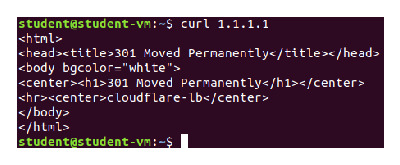
\includegraphics{ip4c.eps}}
	\centering
	\caption{Paket s IPv4 protokolom}
	
	\scalebox{1.3}{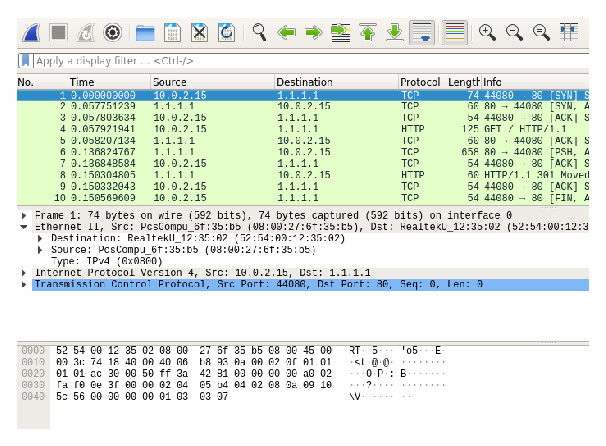
\includegraphics{ip4w.eps}}
	\centering
	\caption{Paket vygenerovaný programom Curl zachytený vo Wireshark}
	
	\scalebox{1.2}{\includegraphics{ip4.eps}}
	\centering
	\caption{Paket vygenerovaný programom Curl zachytený ipk-sniffer}
	\end{figure}
\newpage
	Paket s IPv6 vygenerovaný programom Curl, bohužiaľ jediný spôsob ako bolo možné otestovať podporu IPv6:
	
	\begin{figure}[h]
	\scalebox{1.2}{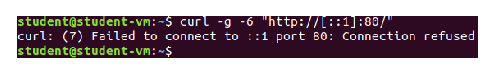
\includegraphics{ip6c.eps}}
	\centering
	\caption{Paket s IPv6 protokolom}
	
	\scalebox{1.3}{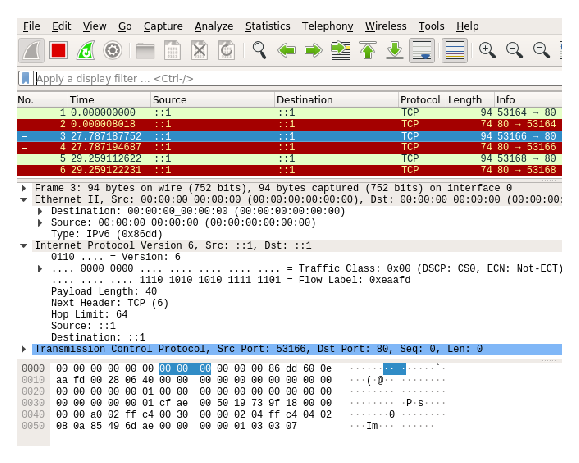
\includegraphics{ip6w.eps}}
	\centering
	\caption{Paket vygenerovaný programom Curl zachytený vo Wireshark}
	
	\scalebox{1.2}{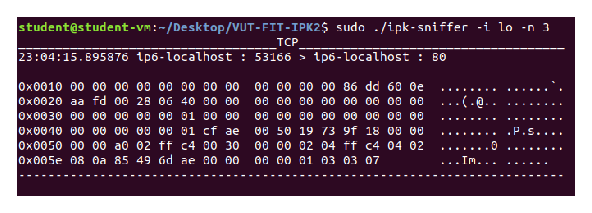
\includegraphics{ip6.eps}}
	\centering
	\caption{Paket vygenerovaný programom Curl zachytený ipk-sniffer}
	\end{figure}
	
	
	\newpage
	\section{Použité zdroje}
	
	\bibliographystyle{czechiso}
	\renewcommand{\refname}{Použitá literatúra}
	\bibliography{manual}
	
	
\end{document}

	
	
	
